\documentclass[tikz]{standalone}
%outline around text
\usepackage[outline]{contour}
\contourlength{1.3pt}

%tikz
\usepackage{tikz}
\usetikzlibrary{knots, cd, calc}


\begin{document}
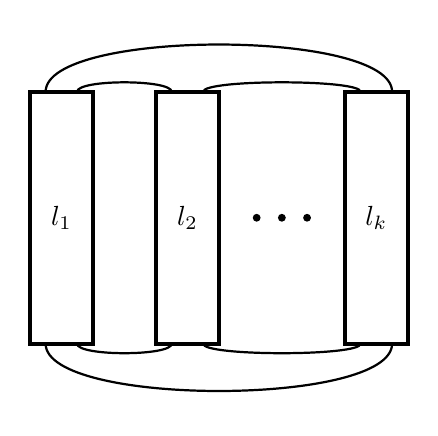
\begin{tikzpicture}[scale = 0.8]
\draw[ultra thick] (0, 0) rectangle (1,4);
\draw[ultra thick] (2, 0) rectangle (3, 4);
\node at (3.6, 2) [circle, fill, inner sep=1pt] {};
\node at (4,2) [circle, fill, inner sep=1pt] {};
\node at (4.4, 2) [circle, fill, inner sep=1pt] {};
\draw[ultra thick] (5, 0) rectangle (6, 4);

\begin{knot}
\strand[thick] (0.25, 4) .. controls +(0, 1) and +(0, 1) .. (5.75, 4);
\strand[thick] (0.75, 4) .. controls +(0, 0.2) and +(0, 0.2) .. (2.25, 4);
\strand[thick] (2.75, 4) .. controls +(0, 0.2) and +(0, 0.2) .. (5.25, 4);

\strand[thick] (0.25, 0) .. controls +(0, -1) and +(0, -1) .. (5.75, 0);
\strand[thick] (0.75, 0) .. controls +(0, -0.2) and +(0, -0.2) .. (2.25, 0);
\strand[thick] (2.75, 0) .. controls +(0, -0.2) and +(0, -0.2) .. (5.25, 0);
\end{knot}

\node at (0.5, 2) {$l_1$};
\node at (2.5, 2) {$l_2$};
\node at (5.5, 2) {$l_k$};
\end{tikzpicture}
\end{document}


